\documentclass[a4paper,12pt]{article}
\usepackage{t1enc}
\usepackage[longnamesfirst, round]{natbib}  % Bindet den natbib-standard fuer das Zitieren ein
\usepackage{epsfig}
\usepackage[utf8]{inputenc}   % Ermoeglicht Sonderzeichen direkt einzugeben
\usepackage[T1]{fontenc}        % Garantiert saubere Worttrennung bei Umlauten etc.
\usepackage{color}              % Farbpaket
\usepackage{amsmath,amsfonts,amssymb}   % ermoeglicht mathematische Sonderzeichen
\usepackage{ngerman}           % neue deutsche Rechtschreibung
\usepackage[english]{babel}     %
\usepackage{ae}                 %
\usepackage{graphicx}           % Ermoeglicht das Einbinden von Bildern in allen Formaten
\usepackage{longtable}          % zum erstellen von Tabellen ber mehrere Seiten
\usepackage{multirow}           % zum Verbinden von Zeilen innerhalb einer Tabelle
%\usepackage{pictexwd}           % PicTex, ein Graphikpaket
%\usepackage{pst-all, multido}   % psTricks, ein Graphikpaket
\usepackage{url}
\usepackage{float}
\usepackage{subcaption}
\usepackage{booktabs, caption}
\usepackage[flushleft]{threeparttable}

% ________________ EINRICHTEN DES DOKUMENTS ______________________%

\bibliographystyle{apalike}    % legt den Stil fuer das Inhaltsverzeichnis fest

\oddsidemargin 0.1in \evensidemargin 0.1in \textwidth 15.5cm \topmargin -0.4in \textheight 24.5cm
\parindent 0cm      % legt die Seitenraender fest

\pagestyle{plain}          % leere Kopfzeile, Seitennummer in der Mitte der Fusszeile

\newcommand{\bs}{\boldsymbol}  % shortcut zur Erzeugung von fetten Sympolen in der Mathe-Umgebung

\renewcommand{\baselinestretch}{1.25}
% 1,5 -facher Zeilenabstand (Standard ist 1,2-facher Zeilenabstand, also 1,2*1,25 = 1,5



\begin{document}

% ________________ TITELSEITE ______________________%


\pagenumbering{roman}   % roemische Zahlen zur Seitennumerierung

\begin{titlepage}       % Umgebung fuer Titelseite, frei gestaltbar

\thispagestyle{empty}   % keine Numerierung auf Titelseite


\begin{center}
\vspace*{2.5cm}
{\bf  \Large Effects of Unemployment Benefits and Uncertainty in Heterogeneous Models\\The Importance of Endogenous Duration of Unemployment} \\
\vspace*{3cm} 
Term paper for the \\ Project Module in Macroeconomics and Public Economics: Uncertainty and Volatility \\
of Prof. Dr. Benjamin Born and Junior-Prof. Dr. Markus Riegler  \\
\vspace*{0.5cm} 
Winter Term 2016/17\\
\end{center}

\vfill
\begin{flushright}
   \emph{Eric Lustenberger} \\
    \emph{Bonner Talweg 34}\\
    \emph{53113 Bonn}\\
   \emph{Stud Nr.: 2849851}\\
 \emph{M.Sc. Economics}\\

\end{flushright}



% 
% \begin{center}
% $ $			% oeffnet und schliesst eine Matheumgebung (Trick, um den Titel nach unten zu rutschen
% \vspace{4cm}
% 
% {\LARGE TITEL}
% \vskip 4cm
% 
% Diese Seite ist frei gestaltbar
% \end{center}

\end{titlepage}

\newpage                % erzwingt an dieser Stelle einen Seitenumbruch



% ________________ INHALTSVERZEICHNIS ______________________%


% \tableofcontents   %fuegt Automatisch ein Inhaltsverzeichnis ein
% 
% \newpage
% 


% ________________ HAUPTTEIL ______________________%


\pagenumbering{arabic}      % Seitenzahlen wieder arabisch numerieren
\setcounter{page}{1}        % Ruecksetzen des Seitenzahlzaehlers auf 1


\section{\"Uberschrift}
\label{Kapitel1}

\subsection{Unter\"Uberschrift}

\subsubsection*{UnterUnter\"Uberschrift}



Hier steht mal ein Text. Eine M\"oglichkeit des Zitierens ist, direkt
im Text die Quelle anzugeben \citep[see][pp.225-369]{key1}.
Andererseits schreiben \cite{key2}, dass man auch so zitieren kann.

In der Matheumgebung kann der oben (im Latex-Quellcode) genannte Shortcut verwendet
werden, um aus einem normalen $\beta$ ein fettes $\bs \beta$ zu
machen. Wichtige Gleichungen, die nochmal verwendet werden, sollten nummeriert werden, z.B.
\begin{equation}
\label{eq:ols}
   b = (x'x)x'y \;.
\end{equation}

Nebens\"achlicheres, auf das man sich nicht mehr bezieht, bleibt unnummeriert, also 
\begin{equation*}
   a = 1\;.
\end{equation*}
Nun kann man direkt auf die erste Gleichung als Gleichung~\eqref{eq:ols} verweisen mittels des zugewiesenen labels. In gleicher Weise kann man auf die Graphik~\ref{fig:ersteGraphik} bzw. Graphik~\ref{fig:andereGraphik} verweisen. Die Tilde zwischen \glqq Graphik\grqq{} und \glqq \verb|\ref{fig:andereGraphik}|\grqq{} verhindert, dass bei Zeilenumbr\"uchen die Zahl als erstes alleine in die neue Zeile rutscht. Ganz analog f\"ur die Tabelle~\ref{tab:Tabelle}. 


\section{Introduction}

In our presentation we have discussed welfare implications of changes in the unemployment policy. We have done so using a simple Aiyagari framework, where agents are subject to exogenous unemployment shocks. These shocks are assumed to be independent of the policy itself. Furthermore, the unemployment rate, which only depends on the different transition probabilities is so too. In other words, changes of the level of unemployment insurance do not affect the unemployment rate. This strongly contradicts empirical literature.\footnote{See \citep{decker} for a review.} The main argument being that higher unemployment benefits will decrease incentives for the workers to look for jobs. Furthermore, there is a great deal of theoretical literature, consisting of search-match and moral hazard models suggesting the same. (cite some guys) 

In the following paper I will depart from the strong assumption of an exogenous job-finding probability, still using the baseline model. Based on the results of an empirical estimation of the relationship between changes in the unemployment rate and the job-finding probability I will let the latter fluctuate with the policy changes. I then show that this may completely change the outcome of the welfare analysis and therefore may have strong policy implications. It may not be sufficient to raise unemployment benefits without undertaking measures to reduce job-finding frictions, such as providing incentives and information to improve the transition from unemployment to employment.

Sections 1 and 2 discuss the model and the welfare analysis, respectively. In section 3 a brief summary of the results presented in class is followed by the analysis, which takes changes in the job-finding probability into account. Finally, section 5 concludes. 


\section{Model}

The setup is a basic \cite{aiyagari} model. The key component of this model is that agents are subject to uninsurable idiosyncratic risk, which hinders their ability to smooth consumption over time. This risk manifests itself in form of a potential income shock agents may experience in each period. In order to insure themselves against such risk, agents accumulate precautionary savings in order to build a buffer for potential future income drops. \\
In contrast to the representative agent model, this mechanism generates a heterogeneous distribution of agents, with different asset levels and different employment status. The heterogeneity opens the door for a number of questions, which remain salient to its representative counterpart. Most importantly, it allows to look at how macroeconomic policy may affect different groups in distinct ways - A policy change may for example be beneficial for the unemployed, while it is harmful for the employed. Moreover, the feature of incomplete insurance, enables us to look at insurance policies. The combination of these features, thus enables us to examine the welfare implications of changes in the unemployment benefits.\\
The following following paragraphs describe the model in a more detailed manner. 

\subsection{Consumer's Problem}

There is a continuum of ex-ante identical (all consumers face the same preferences) infinitely-lived consumers, whereby the population is normalized to 1. In each period consumers choose $ c_{t}$, consumption at time t, and the asset level next period, $k_{i,t+1}$, to maximize the expected discounted lifetime utility: 
\[ 
 max_{\{{ c_{i,t}, k_{i,t+1} }\}_{t = 0}^{\infty}} {\mathbb{E}} \sum_{i=0}^{\infty} \beta^{t}  u(c_{i,t}), 
 \]

where $\beta \in (0,1)$ is the discount factor and $\mathbb{E[\cdot]}$ is the expectation at time 0. In each period, the individual expenditure is constrained by the period income. Consumers thus face to following budget constraint: 
  \begin{equation}
  \label{eq:budconstraint}
  c_{i,t} + k_{i,t+1} = (1 + r_{t} - \delta) k_{i,t} + w_{t} (1 - \tau_{t})  e_{i,t} + \mu w_{t} (1 - e_{i,t}).
 \end{equation} 

$r_{t}$ is the interest rate at time t, $\delta$ is the depreciation rate, $w_{t}(1-\tau_{t})$ is the after-tax wage at time t and $e_{i,t}$ is a dummy variable for the employment status - $e_{i,t}=1$ being employed at time t and $ e_{i,t}=0$ unemployed, respectively. Unemployed consumers receive benefits in form of a replacement rate,$\mu$. Finally, consumers are constrained in their borrowing:
 
   \begin{equation}
  \label{eq:borconstraint}
   k_{i,t + 1} \geq \bar{k}.
 	 \end{equation}
 	 
$\bar{k}$ denotes the minimum amount of capital consumers are required to hold at each point in time.

The employment shocks are governed by an exogenous transition matrix: 
\[ \Pi = \begin{bmatrix}
1-\pi_{UE} & \pi_{UE} \\
 \pi_{EU} & 1-\pi_{EU}
\end{bmatrix}
\]

where $\pi_{UE}$ is the probability to find a job next period and $\pi_{EU}$ is the layoff probability. 

\subsection{Firm's Problem}

The representative firm maximizes profits 
\[ \max_{\substack{K_{t},L_{t}}}F_{t}(K_{t},L_{t})-r_{t}K_{t}-w_{t}L_{t}
\]

Factor prices are obtained by taking the FOC's with respect to the aggregate capital stock and the aggregate labor, respectively: 
\[
r_{t} = \frac{\mathrm d F_{t}(K_{t},L_{t})}{\mathrm d K} = \alpha z (\tfrac{L_{t}}{K_{t}})^{1-\alpha} \]
\[
w_{t} = \frac{\mathrm d F_{t}(K_{t},L_{t})}{\mathrm d L} =(1-\alpha)z (\tfrac{K_{t}}{L_{t}})^{\alpha}
\]

\subsection{The government}

The government runs a balanced budget:
\begin{equation}
  \label{eq:balancedbudget}
\tau_{t}=\mu\frac{1-L_{t}}{L_{t}}
\end{equation}



\subsection{General Equilibrium}

	
	   \begin{equation}
  \label{eq:ssemployment}
   L = \frac{\pi_{UE}}{\pi_{UE}+\pi_{EU}}
 	 \end{equation}

The euler equation is maximizing the consumer's problem
\[ 
c_{i,t}^{- \sigma} \geq \beta (1+r -\delta){\mathbb{E}[c_{i,t+1}^{- \sigma}}]
\]
The households take (current and future) factor prices $r_{t} and w_{t}$ as given. Their policy functions satisfy the first-order conditions and depend on the employment status, wealth and the aggregate state: 
\[ c_{t}(e_{t},k_{t},s_{t}), k_{t+1}(e_{t},k_{t},s_{t})
\]
where $s_{t}$ stands for the aggregate productivity state and the cross-sectional distribution. 

Finally, the aggregated capital and labor must be consistent with aggregate capital and labor used to obtain the factor prices: 
\[ \sum_{i}k_{t+1}(e_{i,t},k_{i,t},s_{t})=K_{t+1}(s_{t}), \ \ \ \sum_{i}e_{i,t}=L_{t} 
\]

\section{Welfare analysis}
We want to compare the utility level of the same agent before and after the policy change. There are two challenges to overcome. Firstly, utility is a purely ordinal measure and therefore not quantifiable. Secondly,we need take transitions into account. It may be the case that during the transition phase from one steady state to the other, agents loose even tough in the end they are in a preferred steady state and therefore do not prefer the policy change taking the transition into account. 

For our presentation we have considered two different forms of welfare measurements - the Consumption equivalent and the Cash equivalent. I will here only discuss the Cash Equivalent. However, the conclusions I will draw from my analysis are the same when using the Consumption Equivalent (See Appendix 1).\footnote{That being said, the two measures differ in the manner they weight different groups. The Consumption equivalent does weight different level's of consumption differently. A concave utility function implies that a consumption change of the same order is weighted differently by rich individuals with a high consumption to poor individuals with a low consumption.} 

\subsubsection*{The Cash Equivalent}

The Cash Equivalent tells you how much cash, as in units of wealth, I have to give to (or take away from) the agent in the first economy, in order for him to be indifferent between the two economies - The two being identical with the exception of two different benefit policies. $U^{1}$ being the lifetime utility in the baseline economy with benefit policy one and $U^{2}$ being the lifetime utility in the economy with the adjusted policy. Formally: 

  \begin{equation}
  U^{2}(e,k) = U^{1}(e,k+\Delta) \nonumber
  \end{equation}

Where $\Delta$ is the transfer of units of wealth in the first period, $e$ is the employment status and $k$ the individual capital. If $ \Delta>0 $ agents prefer the policy change, otherwise they prefer the current state. 

\subsubsection*{Taking transitions into account}

One has to consider the transitions. Approximation used by \cite{KrusellMukoyamaSahin}. Instead of calculating full transitions I compare different steady states, placing the agents along with their capital holding and their employment state into the new economy and I then compare the two lifetime utilities. 




\section{Analysis}

In the following section I will analyze the importance of considering job-search effects when considering changes in the unemployment benefits. How does the welfare analysis change when taking into account that the unemployment duration rises in the benefit level? \\
In order to provide a more detailed welfare analysis, I will look at both the employed and the unemployed when I compare the two cases. Although society on average may clearly favor one particular outcome, it may still be reasonable to implement a certain policy to help the more vulnerable to the detriment of the majority. Typically, the unemployed benefit relatively more from higher benefits than the employed. The latter being in the larger majority, thus leads to the result being biased towards them. 
\\ \\
After I introduce the Calibration, I proceed with a short summary of the results obtained in the baseline case, which corresponds to the results discussed in class.
I then conduct an experiment on the basis of empirical results, which show that an increase in the replacement rate leads to an increase in the unemployment duration. Using this relationship I will recalculate the welfare effects, letting the job-finding probability fluctuate with the benefit level. The second welfare analysis is then compared to the baseline case. 


\subsection{Calibration}

The calibration used here follows \cite{DenHaan20101} is the same as in the presentation, with the small difference, that the transition matrix corresponds to the case with no aggregate risk. The job-finding probability $\pi_{ue}$ therefore takes is slightly higher and takes on the value 0.4 instead of 0.35, which would correspond to the case of a recession when including aggregate risk.\footnote{Since we were also considering aggregate risk in our presentation, we had to chose between the recession and boom state for the Aiyagari calibration and chose the latter. Note, however, that this has no impact on the qualitative result of the welfare analysis.} The calibration is based on quarterly data matching microeconomic data or long-run model considerations. A job-finding probability of 0.4, thus, corresponds to an average unemployment duration of 2.5 quarters or 32.5 weeks. \footnote{Note that here we overestimate the average unemployment duration, since agents remain unemployed for at least one quarter.E.g. \cite{mukoyama} uses a $\pi_{ue}$ leading to an average duration of 17 weeks, which corresponds to post US 1980 economy data.} The discount factor is set at $\beta = 0.99$, productivity at $z = 1$, the capital share at $\alpha = 0.36$, and the depreciation rate $\delta = 0.025$. Finally, the baseline unemployment rate corresponds to  $1- l=0.1$ and the baseline replacement rate is $\mu = 0.15$.

\subsection{Baseline Results}

When we conducted our prior welfare analysis we found that different groups in society want different policies - namely, the unemployed would prefer to change to higher unemployment benefits and the employed would prefer a change to a less re-distributive system. Furthermore, we also found that generally agents do not want full unemployment insurance, although this would clearly eliminate idiosyncratic risk. 
\ref{baseline_ue_vs_e} illustrates this well. 

\begin{figure}
\caption{Results Cash Equivalent Baseline } 
\label{baseline_ue_vs_e}	%label, um spaeter auf die Graphiknummer zugreifen zu koennen
\centering
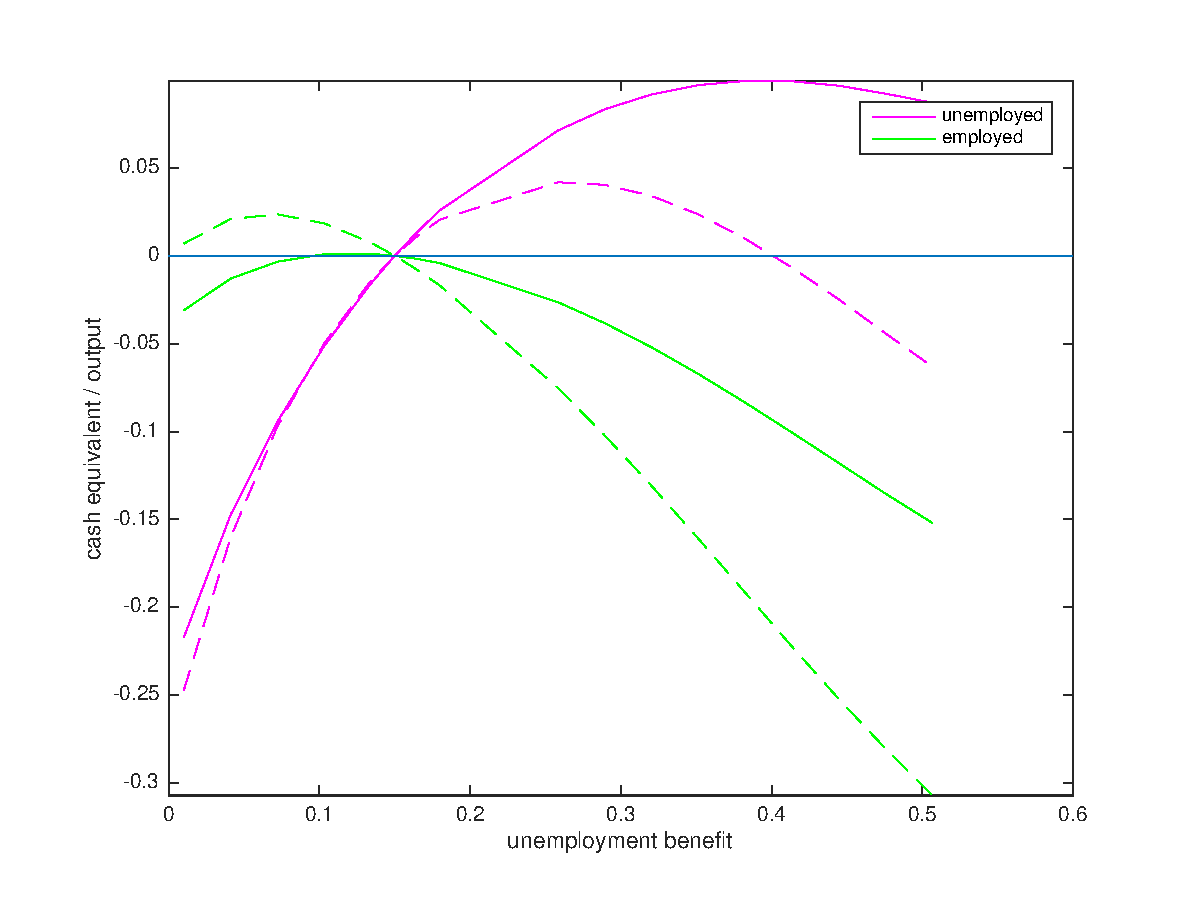
\includegraphics[scale=.5]{Cash_equivalent_baseline}  % width legt Breite der Graphik fest

\begin{minipage}{0.8\linewidth}
\footnotesize{The dotted lines describe the medians and the continues lines the means of the consumption equivalent. The rose lines illustrate the mean and median for the unemployed. The green lines show the consumption equivalent of the mean and median of the employed. The baseline, $\mu = 0.15$, is where the two lines cross. Clearly, the employed prefer lower benefits and the unemployed higher benefits. }
\end{minipage}

\end{figure}

As benefits increase taxes rise to meet the higher demand. Moreover, higher insurance decreases idiosyncratic risk and thus, precautionary savings decrease. This in turn reduces aggregate capital leading to an increase in the return rate on capital and a decrease in wages. 
The employed, thus, experience a sharp decrease in their net-wage, but profit more from higher return rates on capital. The first clearly dominates.\footnote{ (mukoymama working paper.shows that welfare effects are mainly determined by the re-distributional effects of higher taxes and higher benefits. He, however, considers lump-sum taxes and therefore cannot show a different effect for unemployed and employed.} Consequentially the employed prefer a reduction in benefits compared to the baseline level. 
Contrary to the employed, the unemployed receive benefits and are not directly harmed by the changes in the taxes and wages. Furthermore, the richer unemployed, who were able to accumulate savings, also profit from an increase in the return-rates. 
Therefore, they do prefer an increase in benefits. 
Corner solutions (i.e. 0 benefit or the full-insurance case) are both not preferred by either group. Note that taxes also affect the future income of the unemployed, since they have a chance to be employed with a certain probability, this thus reduces future income. The same is true for higher benefits in the case of the employed.\footnote{Net labor income equals unemployment benefits at a replacement rate of 0.9, higher benefits thus would lead to unemployed being better off compared to the employed, which is rather unrealistic.}


\subsection{Endogenizing the job-finding probability}

As discussed above, the transition probabilities and the unemployment rate are exogenously given. In the following analysis I will adapt the job-finding probability with the level of the unemployment benefits. In order for this to affect the unemployment rate, I will fix the job-loss probability, since otherwise the changes of the two transition probabilities would simply cancel each-other out to keep the labor target rate constant.\footnote{One can think of this as a simplified version of the model \cite{mukoyama} uses, abstracting from details regarding job-market rigidities and the Nash bargaining process.} 

I base my calibration on the empirical results. \citep{decker} summarizes the empirical literature, which considers disincentive and incentive effects with respect to changes in unemployment benefits using different approaches as well as a variety of US-samples. He concludes, that a change of 10 percent-points in benefits leads to an extension of the average unemployment duration of 0.5 to 1.5 weeks. 
Thus, I let the job-finding probability such that an 10 percent-point increase of the benefits leads to a prolongation of the average unemployment period of a week. The new job-finding probability is then obtained by the following function:
\begin{equation}
	\pi_{ue}=\frac{1}{x} \nonumber
\end{equation}
where 

\begin{equation}
	x=\cfrac{32.5+\left(\cfrac{\Delta PP \mu}{10}\right)}{13} \nonumber
\end{equation}
is the average unemployment duration in quarters. \\

$32.5$ is the baseline unemployment duration $\Delta PP \mu$ is the percentage point deviation of the unemployment benefits and $\frac{\Delta PP \mu}{10}$ the change in unemployment duration, expressed in weeks.\footnote{Appendix 2 provides a detailed conversion table.} \\
From equation \eqref{eq:ssemployment} follows that the unemployment rate increases as the unemployment duration increases following an increase in unemployment benefits. At the lowest benefit level considered the unemployment rate is at 9.6 percent and the highest benefit the unemployment rate is at 11 percent, with a baseline case of 10 percent. The impact of a change in the replacement rate on the unemployment rate is thus rather small. 

\subsection{Results}


Figure 2 shows displays the mean and median Cash Equivalent for the unemployed and the employed. It clearly shows that all agents prefer lower benefits. While the optimum for the employed lies at 0 (or are negative benefits) the unemployed prefer some benefits, but lower than the baseline. 

\begin{figure}
\caption{Results Cash Equivalent with endogenous job-finding probability} 
\label{baseline_ue_vs_e}	%label, um spaeter auf die Graphiknummer zugreifen zu koennen
\centering
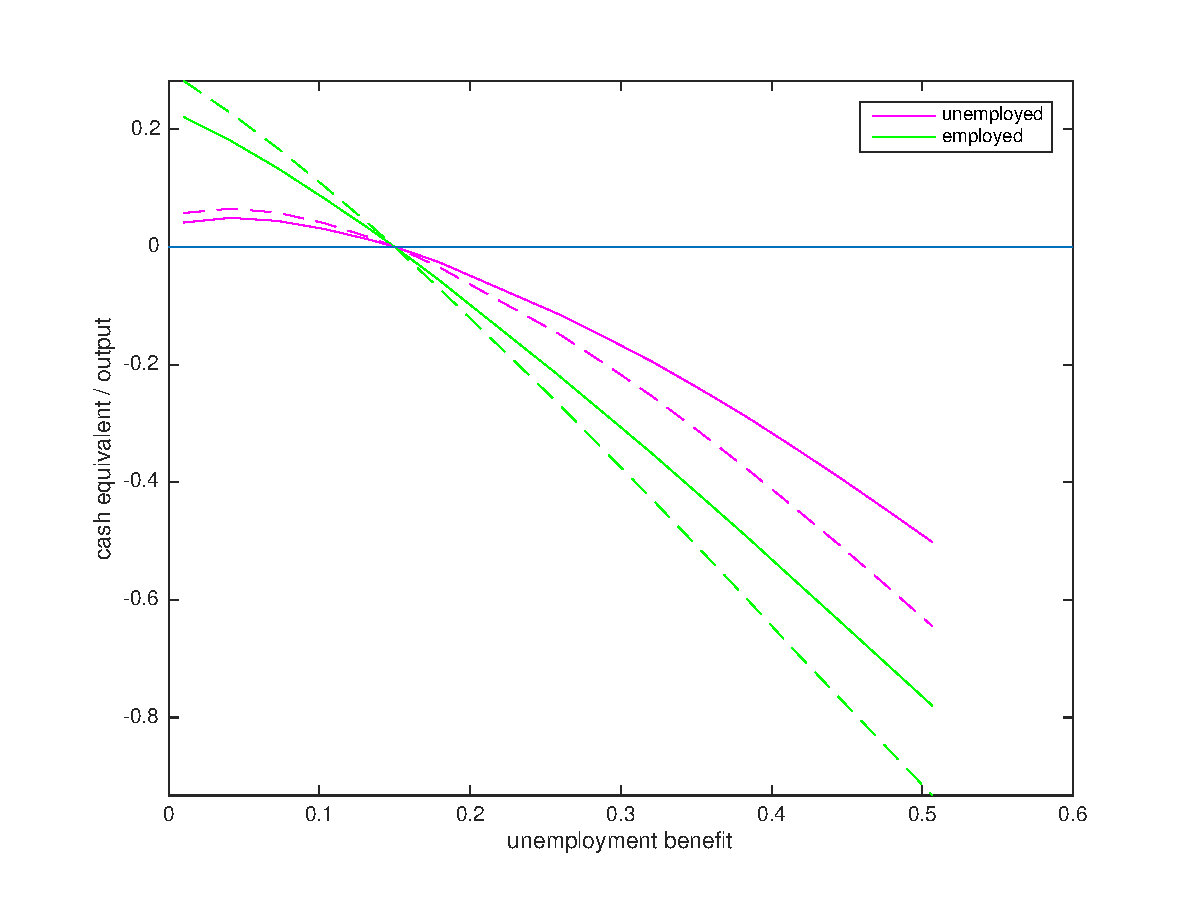
\includegraphics[scale=.5]{cash_equivalent(ue_vs_e)}  % width legt Breite der Graphik fest

\begin{minipage}{0.8\linewidth}
\footnotesize{The dotted lines describe the medians and the continues lines the means of the consumption equivalent. The rose lines illustrate the mean and median for the unemployed. The green lines show the consumption equivalent of the mean and median of the employed. The baseline, $\mu = 0.15$, is where the two lines cross. Clearly, the employed would prefer negative benefits and the unemployed lower benefits. }
\end{minipage}

\end{figure}

Compared to the previous results all agents prefer lower benefits.\footnote{\cite{KrusellMukoyamaSahin} find similar results, when comparing a standard BHA model with a model including endogenous unemployment.} 
As benefits increase the unemployment rate rises. There are therefore less employed who have to pay higher benefits to more unemployed. From equation \eqref{eq:balancedbudget} it follows that taxes will raise to a higher extent than in the previous case since both the unemployment rate and the benefits rise. Thus, the employed will be worse off compared to the baseline case. This amplifying effect works in both directions. As employment increases with lower benefits, the relative taxes decrease faster than in the baseline case and thus, the lowest possible benefits are preferred by the employed. 
While the employed are not directly affected by a change in the transition probabilities, the unemployed's risk of receiving low income increases with an increase in the benefits. Thus their expected future income decreases as they face larger unemployment spells on average. In the present case, this effect seems to be strong enough for the unemployed to prefer to forego some amount of benefits and in turn profit from higher future income prospects on average, as the probability to being employed next period rises. This effect, however, is not strong enough to completely overcome the benefits of a replacement rate and thus in the present case, the unemployed would prefer a $\mu$ of around 0.7. Which also is pareto-optimal, as both, the mean and the median, are maximal at this benefit level. 


\section{Conclusion}

The first observation, thus is, that depending on the model specification one may draw different conclusions when making policy recommendations. Clearly, starting from the baseline calibration describing the US economy, it may make sense to propose a higher benefit-scheme in the first case (the foundation of the argument being, unemployed are better of with higher benefits). However, taking job-search rigidities into account, this line of argumentation clearly fails. 
\\
-> mention that the change in unemployment duration considered is rather small!!! makes result even more astonishing! 
\\
Finally, a policy-scheme simply relying on unemployment benefits is limited. It may be optimal to combine unemployment benefits with reintegration measures facilitating job search and inducing the unemployed to reintegrate themselves in the job market.
Although, the results seem to be similar to those of others, one has to be aware that endogenously determine the transition probability, based on a linear relationship between unemployment duration and unemployment benefits may be limited. First of all this relationship may not be linear (cite some guy). Secondly, higher unemployment benefits may also impact the job-loss probability (cite some guy), although the literature is less clear on that. Finally, I have completely abstracted from a bargaining process, which will also affect the firms side and produce further changes in the wage\citep{mukoyama} for an example. These changes may potentially further alter the results.\footnote{In this simple setting, prices and therefore also the wage, entirely depend on the aggregates driven by individual savings.}  




%_________________ ENDE DES HAUPTTEILS_________________%


\newpage


%_________________ Literaturverzeichnis _______________%

\addcontentsline{toc}{section}{References}        % Fuegt im Inhaltsverzeichnis "References" hinzu
\bibliography{bibexample}                         % Erstellt Literaturverzeichnis (bindet das file bibexample.bib ein

%_________________ Platz fuer Graphiken und Tabellen _______________%

\newpage

% Einfuegen einer Grafik
\begin{figure}
\caption{titel der Graphik} 
\label{fig:ersteGraphik}	%label, um spaeter auf die Graphiknummer zugreifen zu koennen
\centering
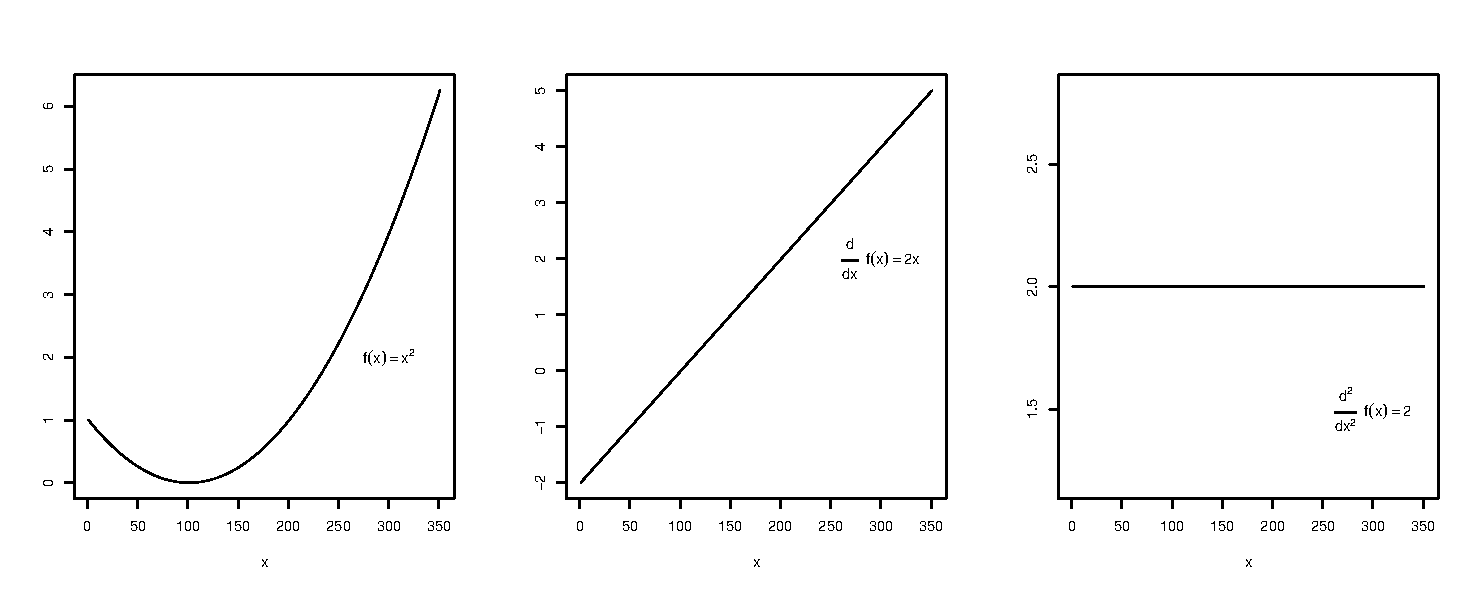
\includegraphics[width=6.5cm]{abb1.png}  % width legt Breite der Graphik fest

\begin{minipage}{0.8\linewidth}
\footnotesize{die Graphik sollte beschrieben werden, sodass man ohne den Text vorne zu lesen wei\ss{}, worum es geht: panel 1 zeigt die Funktion, panel 2 die erste Ableitung und Panel 3 die zweite Ableitung}
\end{minipage}

\end{figure}

\begin{figure}
\caption{titel der Graphik}
\label{fig:andereGraphik} \centering
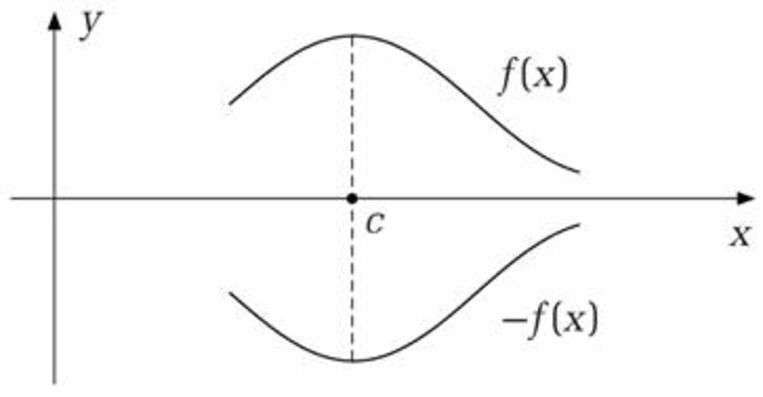
\includegraphics[angle=90,height=6.5cm]{abb2.jpg}  % angle dreht die Graphik, falls noetig; height legt die Hoehe der Graphik fest

\end{figure}

\begin{table}
\caption{Der Title der Tabelle}
\label{tab:Tabelle}
\centering
 \begin{tabular}{lc|r}
   Eine & kleine & Tabelle\\
\hline
   Text links & mittig & oder rechts \\
   & unterstrichen  & \\
\cline{2-2}
   \multicolumn{2}{c|}{\"uber zwei Spalten} & dritte Spalte \\
\end{tabular}   
\end{table}

   





\end{document}
